\documentclass[cn]{homework}

\title{作业9}

\begin{document}
    \maketitle
    \problem[带常数项的随机游走过程]
    设模型为,
    \[y_t=\mu+y_{t-1}+\varepsilon_t,
    \varepsilon_t\overset{\text{i.i.d.}}\sim\mathcal N(0,\sigma^2)\]
    选取$\mu=0.01,\sigma=2$,画出$T=800$期如\cref{fig:seq}。

    \problem[带常数和趋势项的随机游走]
    设模型为,
    \[y_t=\mu+y_{t-1}+\alpha t+\varepsilon_t,
    \varepsilon_t\overset{\text{i.i.d.}}\sim\mathcal N(0,\sigma^2)\]
    选取$\mu=0.01,\alpha=0.001,\sigma=2$,画出$T=800$期如\cref{fig:seq}。


    \problem[带常数项的单位根过程]
    设模型为,
    \[y_t=\mu+y_{t-1}+u_t\]
    这里$u_t$满足 
    \[u_t=0.5u_{t-1}+\varepsilon_t,
    \varepsilon_t\overset{\text{i.i.d.}}\sim\mathcal N(0,\sigma^2)\]
    为一平稳过程。
    选取$\mu=0.01,\sigma=2$,画出$T=800$期如\cref{fig:seq}。

    \begin{figure}[h]
        \centering
        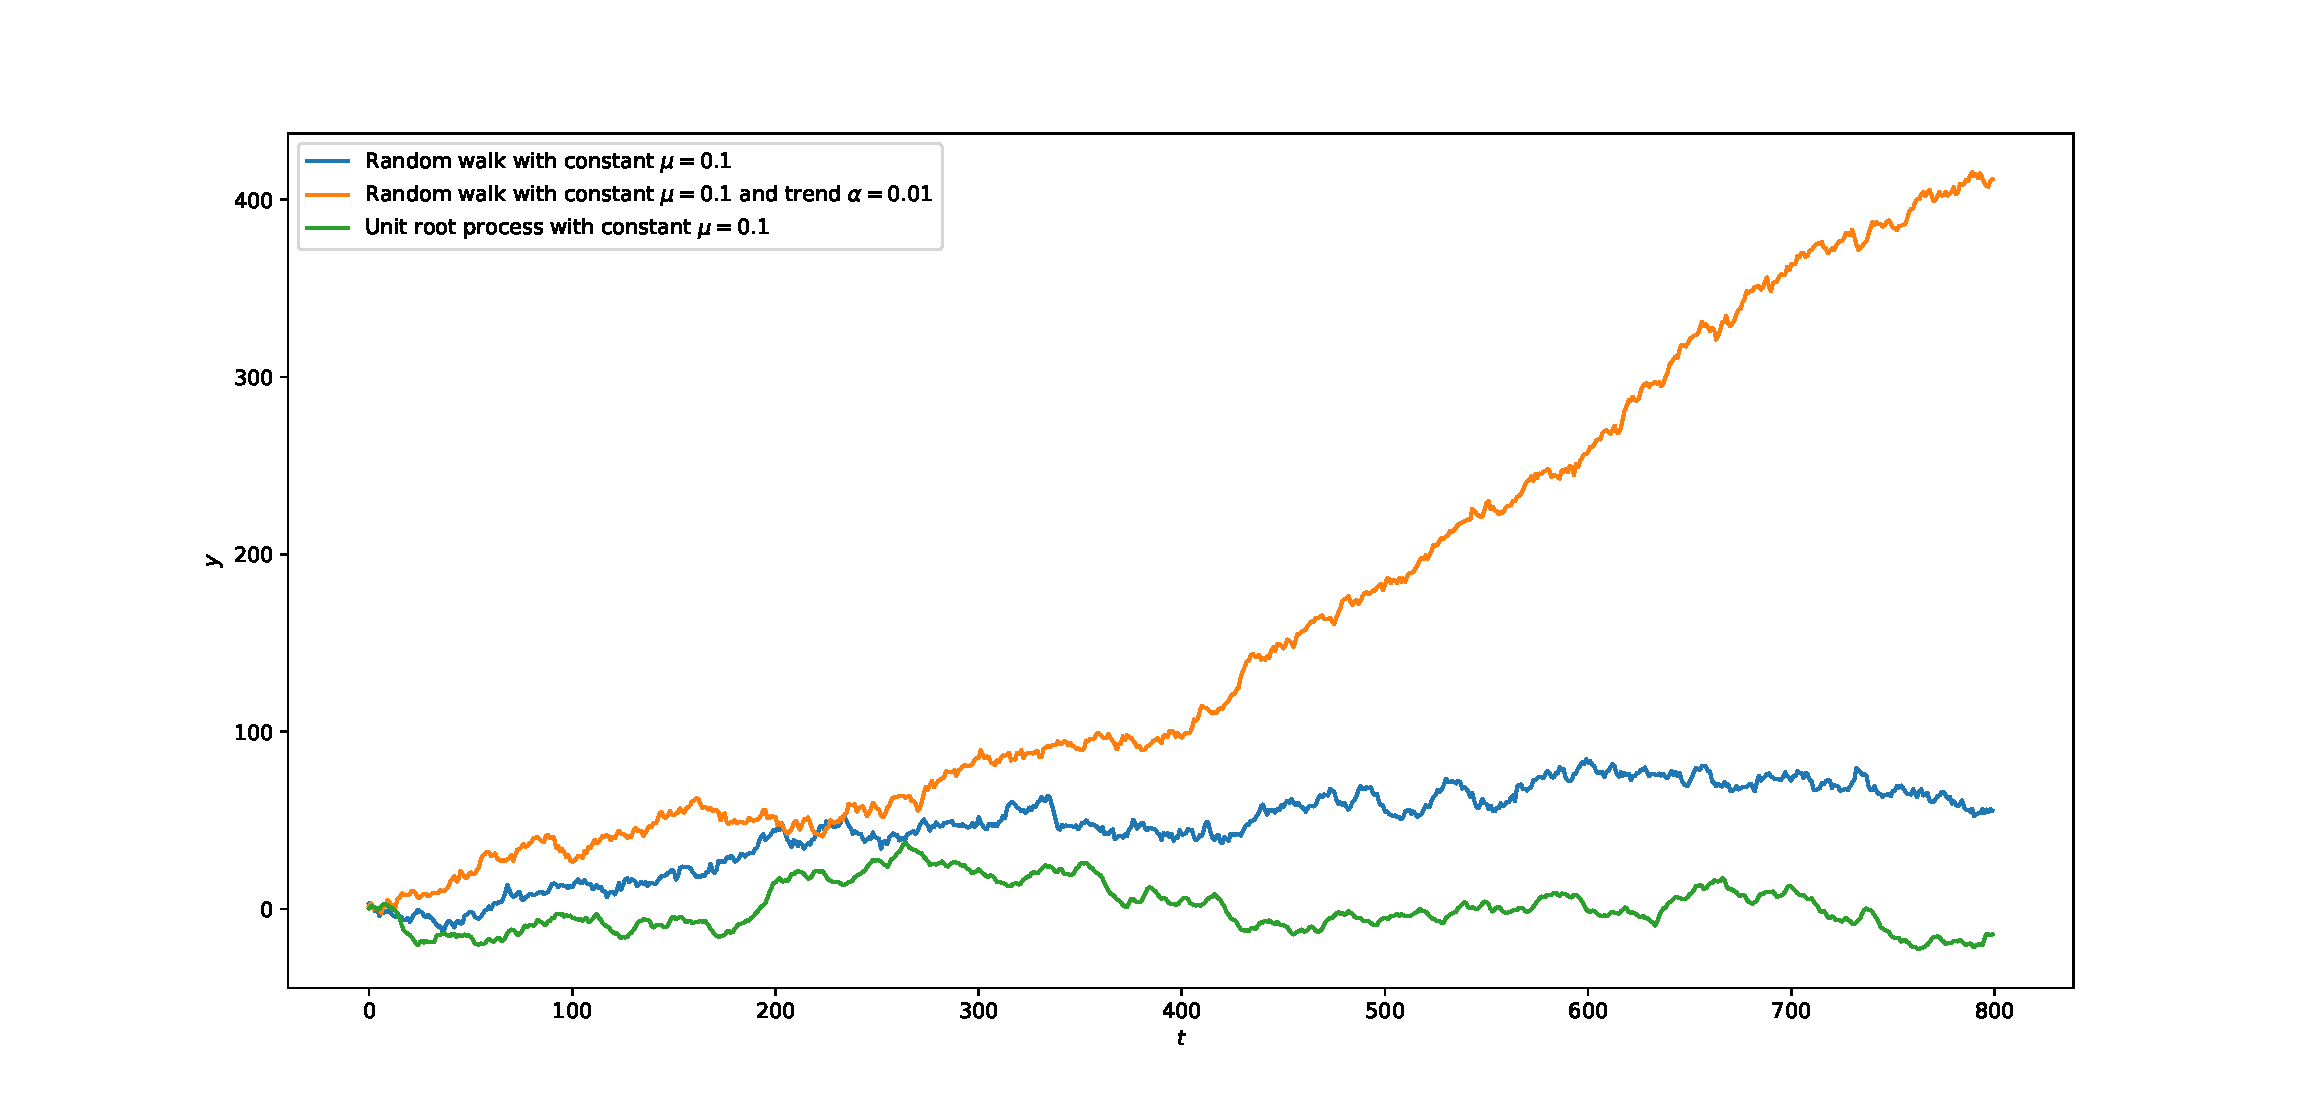
\includegraphics[width=\textwidth]{seq}
        \caption{模拟路径}
        \label{fig:seq}
    \end{figure}

    \problem[第二种情况rho统计量]
    进行10000次模拟得到的直方图如\cref{fig:rho}。
    \begin{figure}[h]
        \centering
        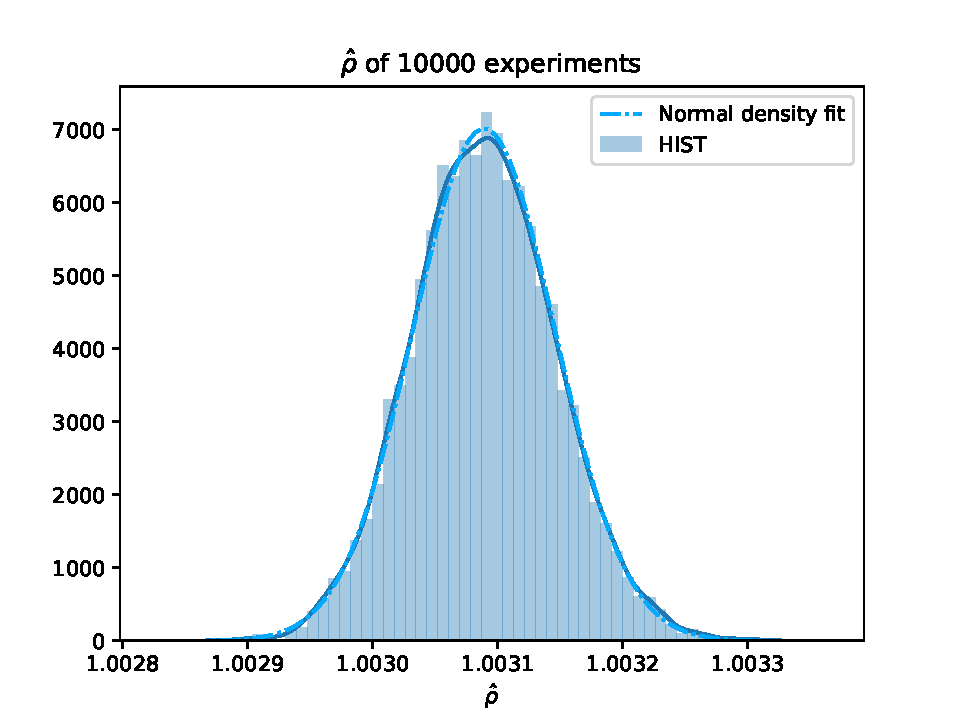
\includegraphics[width=\textwidth]{rho}
        \caption{$\hat\rho$统计量直方图}
        \label{fig:rho}
    \end{figure}

    \newpage
    \appendix
    \section{模拟代码(Python)}
    \lstinputlisting[language=Python]{simulation.py}
\end{document}